% ================================================================================
% Section 1: Introduction with Storytelling Hook (Split Slides)
% ================================================================================
\section{Introduction}

\begin{frame}{Everyone Has Solved Equations, Right?}
    \begin{itemize}
        \item In school, we learn to solve many types of equations:
        \begin{itemize}
            \item \textbf{Linear equations:} $2x + 3 = 7$ \quad (Solution: $x = 2$)
            \item \textbf{Quadratic equations:} $x^2 - 5x + 6 = 0$ \quad (Solutions: $x = 2, 3$)
            \item \textbf{Systems of equations:}
            $\begin{cases}
                2x + y = 5 \\
                x - y = 1
            \end{cases}$
        \end{itemize}
        \item These are familiar problems we've all encountered.
    \end{itemize}
\end{frame}

\begin{frame}{But What If We Restrict to Integers Only?}
    \begin{itemize}
        \item When we require solutions to be \textbf{integers}, we enter a different world.
        \item These are called \textbf{Diophantine equations}, named after Diophantus of Alexandria (3rd century AD).
        \item Example: $x^2 + y^2 = z^2$ has integer solutions: $(3,4,5)$, $(5,12,13)$, etc.
        \item Some equations that have real solutions may have \textbf{no integer solutions} at all!
    \end{itemize}
\end{frame}

\begin{frame}{Now, What If Unknowns Are in the Exponents?}
    \begin{itemize}
        \item This is where it gets really interesting. And we call it,
        \item \textbf{Exponential Diophantine equations:} Unknowns appear in the exponents.
        \item Example: $1 + 5^a = 7^b + 7^c$
        \begin{itemize}
            \item $a,b,c$ are unknown non-negative integers
            \item The bases $5,7,7$ are fixed
        \end{itemize}
        \item These are much harder to solve than polynomial equations.
        \item Our research focuses on the general form:
        \begin{equation}
            1+p^a = q^b + r^c \label{main}
        \end{equation}
        where $p,q,r$ are fixed positive integers.
    \end{itemize}
\end{frame}

\begin{frame}{If You Search on Google...}
    \begin{center}
        \fbox{\begin{minipage}{0.9\textwidth}
            \textbf{Google Search:} "exponential Diophantine equations"
        \end{minipage}}
    \end{center}
\end{frame}

\begin{frame}{If You Search on Google...}
    \begin{center}
        \fbox{\begin{minipage}{0.9\textwidth}
            \textbf{Google Search:} "exponential Diophantine equations"
        \end{minipage}}
    \end{center}
    \begin{figure}
        \centering
        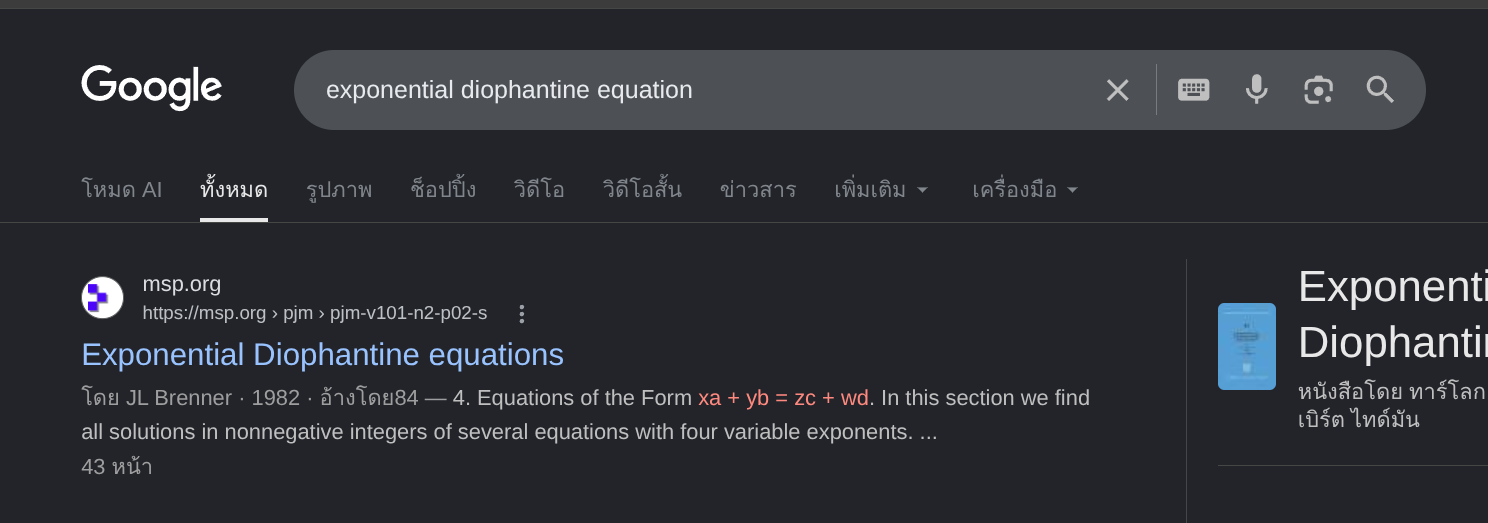
\includegraphics[width=0.7\linewidth]{image.png}
        \label{fig:placeholder}
    \end{figure}
    \begin{itemize}
        \item \begin{block}{Brenner and Foster (1982)}
            "Exponential Diophantine Equations" \\
            \textit{Pacific Journal of Mathematics}, Vol. 101, No. 2, pp. 263-301
        \end{block}
    \end{itemize}
\end{frame}
